\subsection{階層型NNによる学習}
\subsubsection{最適なパラメータを探すためのアプローチ}

まず最初にseed値を1に固定し適当なパラメータの値を決め実行,を繰り返し,その実行結果の中から学習回数が少ないもののパラメータの傾向を探り出しだした.HIDDENを10にすると安定して学習回数が減っているように見えたため,HIDDENを10に固定し,その後今まで試行したもの中から一番学習回数が少なかったETAとalphaの値を元に微調整を繰り返した.\\
上記の方法により以下のパラメータを求めた.\\
\begin{verbatim}
ETA=1.65
ALPHA=0.97
HIDDEN=10
\end{verbatim}

\subsubsection{実行結果}

シー ド値を変えた際の学習収束回数を以下に示す.

\begin{table}[htb]
 \begin{center}
  \caption{階層型NNによるExOR問題の学習に要した回数}
  \label{table:level2}
  \begin{tabular}[htb]{r|l} \hline
   シード値 & 収束した回数 \\ \hline \hline
   1000 & 29 \\ \hline
   2000 & 39 \\ \hline
   3000 & 89 \\ \hline
   4000 & 99 \\ \hline
   5000 & 57 \\ \hline
   6000 & 81 \\ \hline
   7000 & 28 \\ \hline
   8000 & 49 \\ \hline
   9000 & 43 \\ \hline
   10000 & 63 \\ \hline \hline
   10試行の平均値 & 57.7 \\ \hline
  \end{tabular}
 \end{center}
\end{table}

以下に10試行分の学習曲線と,その平均学習曲線を示す.

\begin{figure}[h]
 \begin{center}
  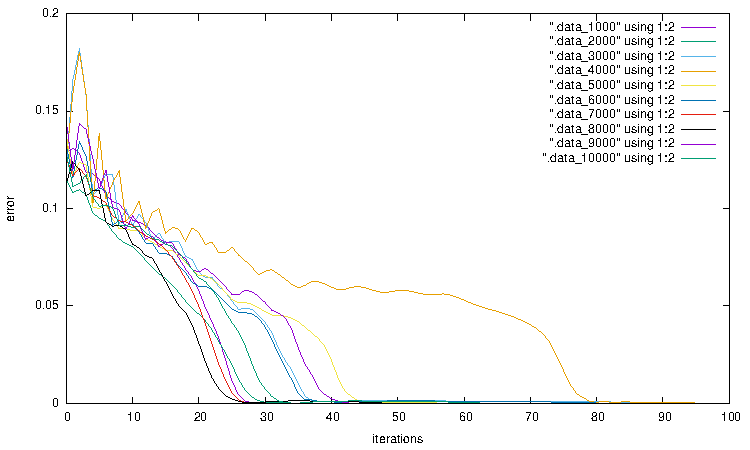
\includegraphics[width=10.0cm]{figs/level2/iterations_vs_error_ave.pdf}
  \caption{seed値1000~10000まで実行したときの結果}
  \label{fig:level2}
 \end{center}
\end{figure}

\begin{figure}[h]
 \begin{center}
  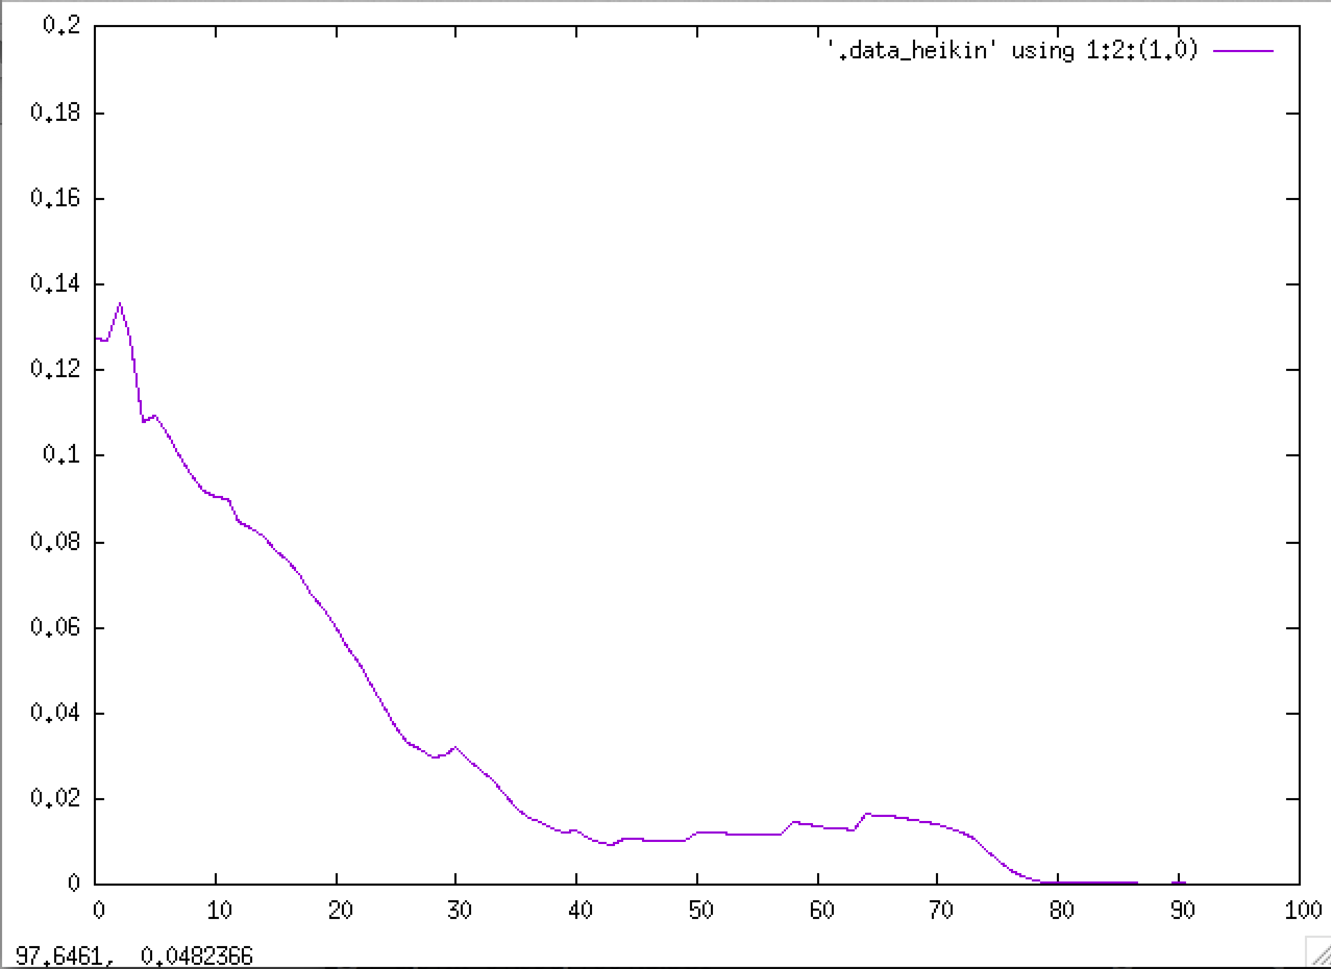
\includegraphics[width=10.0cm]{figs/level2/heikin.pdf}
  \caption{seed値1000~10000まで実行したときの平均}
  \label{fig:level2}
 \end{center}
\end{figure}


\subsubsection{考察}

グラフは,x軸が収束回数,y軸が誤差に対応している.seed値1000~10000まで実行したときの平均のグラフから,平均して誤差が0に限りなく近づくのは,試行回数80~90前後ということがわかる.








